% GNUPLOT: LaTeX picture with Postscript
\begingroup
  \makeatletter
  \providecommand\color[2][]{%
    \GenericError{(gnuplot) \space\space\space\@spaces}{%
      Package color not loaded in conjunction with
      terminal option `colourtext'%
    }{See the gnuplot documentation for explanation.%
    }{Either use 'blacktext' in gnuplot or load the package
      color.sty in LaTeX.}%
    \renewcommand\color[2][]{}%
  }%
  \providecommand\includegraphics[2][]{%
    \GenericError{(gnuplot) \space\space\space\@spaces}{%
      Package graphicx or graphics not loaded%
    }{See the gnuplot documentation for explanation.%
    }{The gnuplot epslatex terminal needs graphicx.sty or graphics.sty.}%
    \renewcommand\includegraphics[2][]{}%
  }%
  \providecommand\rotatebox[2]{#2}%
  \@ifundefined{ifGPcolor}{%
    \newif\ifGPcolor
    \GPcolortrue
  }{}%
  \@ifundefined{ifGPblacktext}{%
    \newif\ifGPblacktext
    \GPblacktexttrue
  }{}%
  % define a \g@addto@macro without @ in the name:
  \let\gplgaddtomacro\g@addto@macro
  % define empty templates for all commands taking text:
  \gdef\gplbacktext{}%
  \gdef\gplfronttext{}%
  \makeatother
  \ifGPblacktext
    % no textcolor at all
    \def\colorrgb#1{}%
    \def\colorgray#1{}%
  \else
    % gray or color?
    \ifGPcolor
      \def\colorrgb#1{\color[rgb]{#1}}%
      \def\colorgray#1{\color[gray]{#1}}%
      \expandafter\def\csname LTw\endcsname{\color{white}}%
      \expandafter\def\csname LTb\endcsname{\color{black}}%
      \expandafter\def\csname LTa\endcsname{\color{black}}%
      \expandafter\def\csname LT0\endcsname{\color[rgb]{1,0,0}}%
      \expandafter\def\csname LT1\endcsname{\color[rgb]{0,1,0}}%
      \expandafter\def\csname LT2\endcsname{\color[rgb]{0,0,1}}%
      \expandafter\def\csname LT3\endcsname{\color[rgb]{1,0,1}}%
      \expandafter\def\csname LT4\endcsname{\color[rgb]{0,1,1}}%
      \expandafter\def\csname LT5\endcsname{\color[rgb]{1,1,0}}%
      \expandafter\def\csname LT6\endcsname{\color[rgb]{0,0,0}}%
      \expandafter\def\csname LT7\endcsname{\color[rgb]{1,0.3,0}}%
      \expandafter\def\csname LT8\endcsname{\color[rgb]{0.5,0.5,0.5}}%
    \else
      % gray
      \def\colorrgb#1{\color{black}}%
      \def\colorgray#1{\color[gray]{#1}}%
      \expandafter\def\csname LTw\endcsname{\color{white}}%
      \expandafter\def\csname LTb\endcsname{\color{black}}%
      \expandafter\def\csname LTa\endcsname{\color{black}}%
      \expandafter\def\csname LT0\endcsname{\color{black}}%
      \expandafter\def\csname LT1\endcsname{\color{black}}%
      \expandafter\def\csname LT2\endcsname{\color{black}}%
      \expandafter\def\csname LT3\endcsname{\color{black}}%
      \expandafter\def\csname LT4\endcsname{\color{black}}%
      \expandafter\def\csname LT5\endcsname{\color{black}}%
      \expandafter\def\csname LT6\endcsname{\color{black}}%
      \expandafter\def\csname LT7\endcsname{\color{black}}%
      \expandafter\def\csname LT8\endcsname{\color{black}}%
    \fi
  \fi
    \setlength{\unitlength}{0.0500bp}%
    \ifx\gptboxheight\undefined%
      \newlength{\gptboxheight}%
      \newlength{\gptboxwidth}%
      \newsavebox{\gptboxtext}%
    \fi%
    \setlength{\fboxrule}{0.5pt}%
    \setlength{\fboxsep}{1pt}%
\begin{picture}(8640.00,5760.00)%
    \gplgaddtomacro\gplbacktext{%
      \csname LTb\endcsname%
      \put(814,704){\makebox(0,0)[r]{\strut{}$0.2$}}%
      \put(814,1236){\makebox(0,0)[r]{\strut{}$0.4$}}%
      \put(814,1769){\makebox(0,0)[r]{\strut{}$0.6$}}%
      \put(814,2301){\makebox(0,0)[r]{\strut{}$0.8$}}%
      \put(814,2833){\makebox(0,0)[r]{\strut{}$1$}}%
      \put(814,3366){\makebox(0,0)[r]{\strut{}$1.2$}}%
      \put(814,3898){\makebox(0,0)[r]{\strut{}$1.4$}}%
      \put(814,4430){\makebox(0,0)[r]{\strut{}$1.6$}}%
      \put(814,4963){\makebox(0,0)[r]{\strut{}$1.8$}}%
      \put(814,5495){\makebox(0,0)[r]{\strut{}$2$}}%
      \put(946,484){\makebox(0,0){\strut{}$0$}}%
      \put(1676,484){\makebox(0,0){\strut{}$0.1$}}%
      \put(2405,484){\makebox(0,0){\strut{}$0.2$}}%
      \put(3135,484){\makebox(0,0){\strut{}$0.3$}}%
      \put(3865,484){\makebox(0,0){\strut{}$0.4$}}%
      \put(4595,484){\makebox(0,0){\strut{}$0.5$}}%
      \put(5324,484){\makebox(0,0){\strut{}$0.6$}}%
      \put(6054,484){\makebox(0,0){\strut{}$0.7$}}%
      \put(6784,484){\makebox(0,0){\strut{}$0.8$}}%
      \put(7513,484){\makebox(0,0){\strut{}$0.9$}}%
      \put(8243,484){\makebox(0,0){\strut{}$1$}}%
    }%
    \gplgaddtomacro\gplfronttext{%
      \csname LTb\endcsname%
      \put(176,3099){\rotatebox{-270}{\makebox(0,0){\strut{}Histogram}}}%
      \put(4594,154){\makebox(0,0){\strut{}$|\cos(\measuredangle(\va{b},\va{T}_i))|$}}%
      \csname LTb\endcsname%
      \put(4246,5322){\makebox(0,0)[r]{\strut{}Q10: $H(|\cos(\measuredangle(\delta \va{b},\va{T_1}))|)$}}%
      \csname LTb\endcsname%
      \put(4246,5102){\makebox(0,0)[r]{\strut{}Q10: $H(|\cos(\measuredangle(\delta \va{b},\va{T_2}))|)$}}%
      \csname LTb\endcsname%
      \put(4246,4882){\makebox(0,0)[r]{\strut{}Q10: $H(|\cos(\measuredangle(\delta \va{b},\va{T_3}))|)$}}%
      \csname LTb\endcsname%
      \put(4246,4662){\makebox(0,0)[r]{\strut{}Q10: $H(|\cos(\measuredangle(\delta \va{b},\va{\omega}))|)$}}%
      \csname LTb\endcsname%
      \put(4246,4442){\makebox(0,0)[r]{\strut{}Q02: $H(|\cos(\measuredangle(\delta \va{b},\va{T_1}))|)$}}%
      \csname LTb\endcsname%
      \put(4246,4222){\makebox(0,0)[r]{\strut{}Q02: $H(|\cos(\measuredangle(\delta \va{b},\va{T_2}))|)$}}%
      \csname LTb\endcsname%
      \put(4246,4002){\makebox(0,0)[r]{\strut{}Q02: $H(|\cos(\measuredangle(\delta \va{b},\va{T_3}))|)$}}%
      \csname LTb\endcsname%
      \put(4246,3782){\makebox(0,0)[r]{\strut{}Q02: $H(|\cos(\measuredangle(\delta \va{b},\va{\omega}))|)$}}%
    }%
    \gplbacktext
    \put(0,0){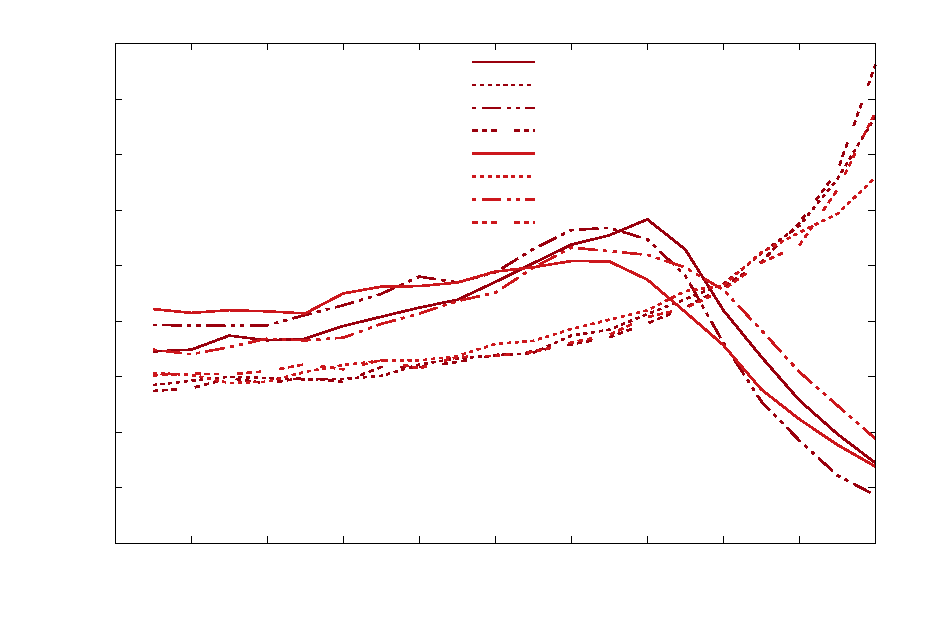
\includegraphics{figures/histograms/mhd_strain_magnetic_angle_histo_t20}}%
    \gplfronttext
  \end{picture}%
\endgroup
